\documentclass[italian]{article}

\usepackage{amsmath}
\usepackage{graphicx}
\usepackage{ragged2e}
\usepackage{lipsum}
\usepackage{float}
\usepackage{hyperref}
\usepackage{tikz}
\usepackage{caption}
\usepackage{listings}
\usepackage{color}
\usepackage{ amssymb }
\usepackage{xcolor}

\definecolor{codegreen}{rgb}{0,0.6,0}
\definecolor{codegray}{rgb}{0.5,0.5,0.5}
\definecolor{codepurple}{rgb}{0.58,0,0.82}
\definecolor{backcolour}{rgb}{0.95,0.95,0.92}

\lstdefinestyle{mystyle}{
    backgroundcolor=\color{backcolour},   
    commentstyle=\color{codegreen},
    keywordstyle=\color{magenta},
    numberstyle=\tiny\color{codegray},
    stringstyle=\color{codepurple},
    basicstyle=\ttfamily\footnotesize,
    breakatwhitespace=false,         
    breaklines=true,                 
    captionpos=b,                    
    keepspaces=true,                 
    numbers=left,                    
    numbersep=5pt,                  
    showspaces=false,                
    showstringspaces=false,
    showtabs=false,                  
    tabsize=2
}

\title{%
  \textbf{Tecniche di parallel computing} \\
  \large algoritmi paralleli in C++ per la risoluzione \\
    di PDE in ambiente openMP, MPI e DEAL II}
\date{}
\author{Omar Kahol\\1162382}
\makeindex


\begin{document}
\noindent\makebox[\textwidth][c]{%
\begin{minipage}[t][0pt]{\linewidth}
\begin{figure}[H]
\centering
  
\includegraphics[width=0.2\linewidth]{unipd.jpeg}
\end{figure}
\centering

UNIVERSITÀ DEGLI STUDI DI PADOVA\\
FACOLTÀ DI INGEGNERIA\\
CORSO DI LAUREA IN INGEGNERIA AEROSPAZIALE

\maketitle

\begin{figure}[H]
\centering
  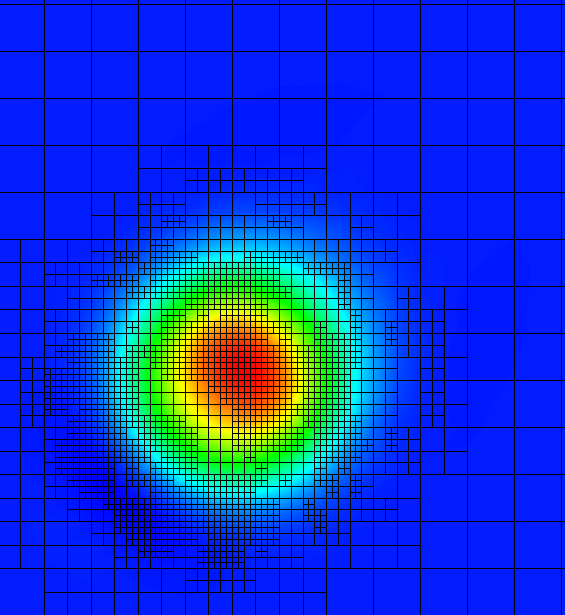
\includegraphics[width=0.5\linewidth]{immagine_iniziale.png}
\end{figure}

\bigskip
Tesi di laurea in Aerodinamica
\end{minipage}}
\newpage
\justifying

\section{INTRODUZIONE}
La risoluzione di problemi ingegneristici è spesso legata ad un insieme di modelli matematici che si presentano in forma di equazioni differenziali alle derivate parziali. Tali modelli devono essere convalidati e risolti per poter ottenere dei risultati utili per le analisi successive. Nel caso dell’aerodinamica lo studio delle interazioni tra un corpo e il fluido è modellato da un sistema di PDE che prende il nome di sistema di equazioni di Navier-Stokes. Di seguito è riportata l’equazione di conservazione della quantità di moto.

\begin {equation*}
\rho(\frac{\partial \vec{u}}{\partial t}+(\vec{u}\cdot \nabla)\vec{u}) = -\nabla p + \rho \vec{f} + \mu \nabla^2 \vec{u}
\end{equation*}

Tralasciando il problema della validazione del modello, si può certamente affermare che una soluzione analitica, assegnato un dominio $\Omega$ e delle condizioni al contorno sulla sua frontiera $\partial \Omega$, in generale non esiste. Si è quindi costretti a procedere mediante metodi risolutivi numerici. In questo elaborato verrà presentato sia il metodo delle differenze finite che il metodo degli elementi finiti. La filosofia che sta alla base della maggior parte di questi metodi è quella di “riduzione dei gradi di libertà della soluzione cercata”:
\\se consideriamo il sistema di equazioni di Navier-Stokes, la soluzione (considerando solamente l’incognita velocità) in un dominio arbitrario, si esprime mediante una funzione $\vec{u}(\vec{x},t)$
che risolve il sistema di equazioni in tutti i punti interni al dominio e rispetta le condizioni nei punti della frontiera. Tale soluzione analitica può essere vista come un insieme di $\infty^n$ parametri liberi. Ciò significa che possiamo immaginare che per descrivere completamente una funzione $f(x,t)$ ci sia bisogno di un numero infinito di valori corrispondenti esattamente al numero di punti della dimensione spaziale e temporale. La semplificazione attuata dai modelli numerici consiste “nell’accontentarsi” di un insieme non infinito di parametri. Ad esempio potremmo esprimere la soluzione come un numero di $Nx \cdot Ny \cdot Nz \cdot Nt$ parametri liberi, in cui le $N$ rappresentano il numero di parametri assegnati ad una particolare dimensione. Nel metodo delle differenze finite tali parametri sono i punti in cui si risolve l’equazione e nel metodo degli elementi finiti tali parametri sono il numero di iterazioni temporali e il numero di celle in cui è stato suddiviso il dominio. È importante notare che la soluzione numerica non è  una interpolazione della soluzione analitica nei punti del dominio e questo ci permette di cercare la soluzione approssimata mediante la risoluzione di problemi che saranno quindi diversi, più semplici, della PDE.\\
Se il problema è ben posto allora l’errore diminuisce all’aumentare del numero di parametri scelti. Ciò ci spinge, per ottenere risultati sempre più precisi, ad avere un numero molto elevato di parametri liberi e a lasciare che sia l’enorme potenza di calcolo di un computer a risolvere il problema numerico. Il problema consiste nel fatto che un programma viene tipicamente eseguito in maniera sequenziale, ciò significa che la CPU esegue un'unica operazione alla volta. Un codice numerico che implementa questo tipo di approccio è detto seriale. Questa limitazione non è un problema per una buona percentuale di problemi considerato che il numero di operazioni che possono essere svolte in un secondo è molto elevato; però, in alcuni un codice seriale risulta essere troppo lento e quindi inadatto e poco efficiente. Questo elaborato intende quindi presentare un modo alternativo di risolvere tali problemi che consiste nella suddivisione del carico computazionale a più processori. Due approcci sono dunque possibili:
\begin{enumerate}
\item[1)] Memoria condivisa, cioè le macchine hanno libero accesso agli stessi dati. L'implementazione sfrutta l'ambiente openMP che consiste in una serie di direttive al preprocessore che permettono di parallelizzare in modo automatico una serie di istruzioni seriali.
\item[2)]Memoria distribuita, cioè ogni macchina dispone della sua memoria non condivisa. La comunicazione avviene tramite uno scambio di informazioni. L'interfaccia utilizzata per implementare questo standard è MPI (Message Passing Interface) ovvero una libreria che implementa una serie di funzioni che permette lo scambio di dati tra processi differenti.
\end{enumerate}

\section{PROCEDIMENTO ADOTTATO}
Le tecniche di parallel computing discusse sono state implementate per risolvere il seguente problema:
\begin{equation*}
\frac{\partial u}{\partial t} + (\vec{c} \cdot \nabla)u = k \nabla ^ 2 u    
\end{equation*}
al quale sono state imposte condizioni al contorno periodiche in modo tale da rendere l'insieme $\Omega$ in cui è definita la soluzione un anello, per il caso monodimensionale, e un toroide nel caso bidimensionale.\\
La scelta del problema è giustificata dalla sua semplicità (in alcuni casi esiste anche una soluzione analitica) che ha quindi permesso un maggiore focus alla parallellizzazione del codice (piuttosto che alla codifica) ma anche dalla somiglianza con l'equazione della quantità di moto della meccanica dei fluidi. Sì può notare infatti la presenza di un termine diffusivo e di un termine convettivo (che in questo caso è lineare).\\
Il linguaggio utilizzato è il C++ perchè supporta pienamente entrambi gli standard openMP e MPI, è compilato quindi molto veloce, è un linguaggio ad oggetti e per questo motivo si presta molto per la risoluzione di codici scientifici ed è efficiente nella gestione della memoria. Tutti i codici prodotti sono disponibili su GitHub:\\
\url{https://github.com/omi14098/Parallel-PDE-solvers}\\
I codici prodotti sono stati raggruppati in questo modo

\begin{enumerate}
\item[1.] DIFFERENZE FINITE
\begin{enumerate}
\item[1.1] 1D
\begin{enumerate}
\item[1.1.1] OPENMP
\item[1.1.2] MPI
\end{enumerate}
\item[1.2] 2D
\begin{enumerate}
\item[1.1.1] OPENMP
\item[1.1.2] MPI
\end{enumerate}
\end{enumerate}
\item [2.] ELEMENTI FINITI
\end{enumerate}
Il metodo delle differenze finite è semplice da implementare e per questo motivo è stato scelto per illustrare i meccanismi di un codice parallelo. Tutte le funzioni, tranne quelle della standard template library, sono state codificate in maniera indipendente, senza l'ausilio di librerie esterne. L'implentazione in 2D verrà usata per estendere il concetto di suddivisione del dominio in MPI e le tecniche di allocamento della memoria. Il codice che sfrutta il metodo degli elementi finiti è stato invece concepito per fornire una implementazione robusta e flessibile di un solver parallelo. Per fare ciò si è fatto un uso di librerie esterne. Quella principale è DEAL II che, attraverso dei wrapper per un insieme di altre librerie (prima fra tutte PETSc per l'implementazione di algoritmi paralleli per l'algebra lineare), offre un ambiente comodo per la risoluzione di PDE. Un codice in DEAL II ha la caratteristica di essere:
\begin{enumerate}
\item[1] efficiente, perchè gli algoritmi sono sviluppati, aggiornati e testati molto spesso da un insieme di contributers.
\item[2] flessibile, perchè l'elevata modularità permette di poter aggiugere o rimuovere funzionalità senza dover riscrivere la maggior parte del codice.
\item[3] completo, perchè le features che possono essere implementate sono in numero maggiore rispetto a quelle che è possibile implementare in autonomia.
\item[4] ben documentato.
\end{enumerate}
Per questo motivo il codice FEM risolve il problema analizzato implementando le seguenti features:
\begin{enumerate}
\item[1] \textbf{DIMENSION INDIPENDENCE} = l'implementazione è, grazie all'utilizzo dei templates del linguaggio C++, pressochè indipendente dalla dimensione del dominio fisico in cui è definita la soluzione.
\item[2] \textbf{ADAPTIVE MESHING} = ogni $n$ iterazioni temporali la mesh viene modificata in modo tale da essere più fitta nelle zone in cui la stima dell'errore è maggiore.
\item[3] \textbf{MPI} = parallelizazione completa utilizzando dei wrapper per le librerie PETSc che implementano degli algoritmi per svolgere operazioni di algebra lineare in parallelo con MPI.
\end{enumerate}

\section{PARALLEL DESIGN PATTERNS}
In un codice possono esistere due tipi di parallelismo
\begin{enumerate}
\item[1] IMPLICITO, cioè la suddivisione del carico computazione non è a carico del programmatore. Il parallelismo può essere il risultato del linguaggio utilizzato (linguaggi di alto livello) o del compilatore scelto. Questo ha il vantaggio di semplificare l'implementazione ma rende i bug più difficili da risolvere e peggiora l'efficienza del programma.
\item[2] ESPLICITO, cioè la parallellizzazione avviene mediante costrutti o annotazioni, che sono al di sopra del linguaggio utilizzato, che devono essere invocati in maniera esplicita dal programmatore. Il programma è potenzialmente sia molto efficiente che molto difficile da debuggare.
\end{enumerate}
Una ulteriore classificazione delle tipologie, a livello hardware, del parallelismo è esplicata dalla tassonomia di Flynn. Più precisamente, tale classificazione interessa l'hardware dei calcolatori che però influenza il tipo di algoritmo parallelo che deve essere scritto. La tassonomia di Flynn individua come parametri fondamentali i seguenti:
\begin{enumerate}
\item INSTRUCTION, cioè il numero di istruzioni differenti che vengono eseguite. Un sistema può essere o single o multiple instruction
\item DATA, cioè il numero di dati dversi elaborati. Un sistema può essere o single o multiple data.
\end{enumerate}
Quindi i tipi di elaboratori considerati sono i seguenti
\begin{enumerate}
\item SISD [single instruction single data] = l'hardware non implementa nessun tipo di parallelismo. Questo significa che il processore esegue una istruzione alla volta su un unico stream di dati. I programmi seriali possono essere elaborati da questo tipo di architettura.
\item MISD [multiple instruction single data] = architettura che non trova, litatamente all'interesse di questo elaborato, applicazioni pratiche.
\item SIMD [single instruction multiple data] = l'elaboratore esegue un'unica istruzione su diversi stream di dati. È il tipico modello di GPU.
\item MIMD [multiple instruction multiple data] = parallelizzazione totale a livello di dati elaborati ed istruzioni eseguite.  Ciò significa che ogni processore esegue una istruzione diversa su flussi di dati diversi ovvero il problema viene diviso in sottoproblemi. A seconda del modo in cui avviene lo scambio di informazioni tra i processori si ha la seguente classificazione:
\begin{enumerate}
\item SISTEMI A MEMORIA CONDIVISA - I processori lavorano in maniera asincrona condividendo una parte della memoria. Questo è il tipo di architettura che viene sfruttata dai codici in openMP. La comunicazione avviene mediante la sincronizzazione (perdita parziale dell'asincronia) delle operazioni.
\item SISTEMI A MEMORIA DISTRIBUITA - I processori lavorano in maniera asincrona su pool di dati differenti. La comunicazione avviene mediante uno scambio di informazioni sincronizzato. Gli standard MPI (message passing interface) permetto di eseguire codice su queste architetture.
\end{enumerate}
\end{enumerate}

Un cluster di elaboratori ha la seguente struttura.
\begin{figure}[h!]
\centering
  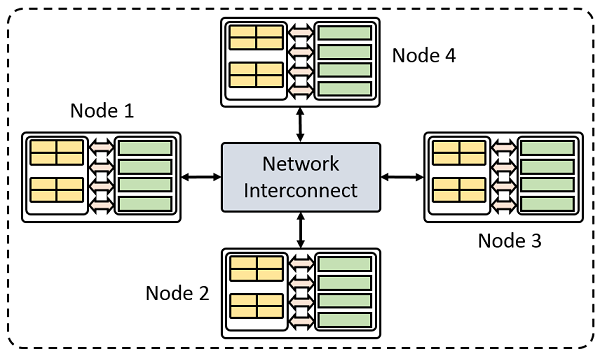
\includegraphics[width=0.6\linewidth]{smp.png}
  \caption*{\tiny \url{https://cdn.comsol.com/wordpress/2014/10/Model-of-cluster.png}}
\end{figure}

Ogni nodo consiste in un elaboratore a memoria condivisa.

\begin{figure}[h!]
\centering
  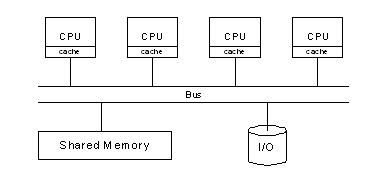
\includegraphics[width=0.6\linewidth]{SMP.JPG}
  \caption*{\tiny \url{https://static.usenix.org}}
\end{figure}

Ogni processore dispone di una memoria privata, detta cache, e di una connessione attraverso una interfaccia ad una memoria condivisa. Le operazioni di I/O sono anch'esse sincronizzate da un interfaccia ma non riguardano questo elaborato. È importante notare che le cache possono essere anche condivise da più processori. Questo fatto porta a delle spiacevoli conseguenze che un codice shared memory non può permettersi di ignorare. Le conseguenze sono due 
\begin{enumerate}
\item[1] DATA RACE = Una variabile presente nella memoria condivisa e utilizzata da due processi diversi viene caricata nelle rispettive cache dei due processori. A questo punto ogni modifica effettuata da un processore non è visibile all'altro, si dice cioè che i processori non hanno una "consistent view" della memoria. È immediato concludere che non è possibile avere più processi che effettuano operazioni di read e write sulla stessa variabile.
\item[2] FALSE SHARING = Questo fenomeno si verifica soprattutto quando si opera con array. Se due processori lavorano su due variabili indipendenti che sono però sulla stessa cache line allora ogni modifica di una variabile invalida automaticamente l'altra, nonostante siano indipendenti. Ciò costringe il secondo processore ad effettuare una operazione di read e ciò diminuisce il livello di asincronismo del programma che rischia di diventare seriale.
\end{enumerate}
Si evince che il modo in cui vengono gestite le operazioni di read e write gioca un ruolo fondamentale nella corretta esecuzione del programma. Il programma scritto dal programmatore contiene una serie di istruzioni Read e Write ordine secondo uno schema logico ben definito. Il compilatore può scegliere di mantenere tale ordine (sequential consistency) oppure di cambiarlo (relaxed consistency). Per ragioni legate alla performance, l'output del compiler (questo vale per i comiplatori C++ usati in questo programma ovvero "mpicxx compiler" e "GNU C compiler") riordina le operazioni di read e write. OpenMP, ad esempio, permette di forzare in un punto qualsiasi del programma le operazioni di read e write. Detto ciò, è importante prestare molta attenzione alle operazioni di sincronizzazione (per evitare data race) e alle operazioni di memory allocation (se si lavora su array o su std::vector). Da questo punto di vista l'ambiente openMP offre delle funzioni che gestiscono questi procedimenti.


\section{IL METODO DELLE DIFFERENZE FINITE}
Il problema 1D è il seguente.
$$\begin{cases}
\frac{\partial u}{\partial t} + c \frac{\partial u}{\partial t} = k \frac{\partial ^ 2 u}{\partial x ^ 2}, u(x,t) \in (0,1) \times (0,1)
\\ u(0,t) = u(1,t)
\\ \frac{\partial u}{\partial x}(0,t) = \frac{\partial u}{\partial x}(1,t)
\\ u(x,0) = \sin (2 \pi x), x \in [0,1]
\end{cases}$$
Per la particolare scelta di condizione iniziale, esiste una soluzione analitica
$$u(x,t) = sin(2 \pi (x-ct)) \cdot e ^ {-k {2 \pi}^{2} t}$$
Una giustificazione naive è la seguente.\\
La funzione a variabili separabili $u(x,t) = sin(2 \pi x) \cdot e ^ {-k {2 \pi}^{2} t}$ risolve il problema diffusivo. L'equazione del trasporto ha come soluzione $u(x,t) = u_0 (x-ct)$ quindi l'idea sta nel combinare i due effetti. Il termine esponenziale ha quindi l'effetto di "diffondere" $u(x,t)$ e il termine sinusoidale la trasporta. 
\bigskip

La soluzione numerica con il metodo delle differenze finite prevede inizialmente la discretizzazione dell'operatore derivata temporale. Le modalità più elementari sono
\begin{enumerate}
\item[1] ESPLICITO $$\frac{u^{n+1}-u^{n}}{\Delta t} = \mathcal{L}(u^{n})$$
\item[2] IMPLICITO $$\frac{u^{n+1}-u^{n}}{\Delta t} = \mathcal{L}(u^{n+1})$$
\end{enumerate}
È naturale chiedersi se e per quali scelte di $\Delta t$ le soluzioni ottenute saranno stabili. Per rispondere a questa domanda è necessario però fornire una classificazione del modello, in particolare sappiamo che tale equazione ha un carattere iperbolico (dato dal termine convettivo) e un carattere parabolico (dato dal termine diffusivo). Si dimostra che il metodo implicito è sempre stabile mentre quello esplicito necessita di uno step temporale deve essere proporzionale alla finezza della discretizzazione spaziale, cioè $\Delta x$, nel caso di problemi iperbolici e al suo quadrato, nel caso di problemi parabolici. Il metodo implicito sembra quindi essere la scelta migliore però il metodo esplicito è più semplice dal punto di vista dell'implementazio e per questo motivo è stato preferito. Per la scrittura del codice in DEAL.II ho considerato altre alternative ovvero:
\begin{enumerate}
\item[1] IMEX cioè usare un metodo implicito per trattare il termine parabolico e un metodo esplicito per il termine iperbolico.
$$\frac{u^{n+1}-u^{n}}{\Delta t} + \vec{c} \cdot \nabla u^n = k \nabla ^ 2 u^{n+1}$$
\item[2] $\theta$-SCHEME ovvero 
$$\frac{u^{n+1}-u^{n}}{\Delta t} = \mathcal{L}(\theta u^{n+1} + (1-\theta)u^n)$$
\end{enumerate}
E ho scelto un $\theta$-SCHEME con $\theta=0.5$.
Dalla scelta della discretizzazione spaziale si ottiene il seguente problema
$$\frac{u^{n+1}_i-u^{n}_i}{\Delta t} + c \frac{u^n_{i+1}-u^n_{i-1}}{2 \Delta x} = k \frac{u^n_{i+1}-2u^n_i+u^n_{i-1}}{\Delta x ^ 2}$$
In questa scrittura i e n corrispondono ai gradi di libertà della dimensione spaziale e temporale ovvero $i=1..N_x$ e $n=1..N_t$. L'incognita del problema è quindi $u^{n+1}_i$ e può essere calcolata direttamente con due cicli for. 
\subsection{LA STRUTTURA DEL PROGRAMMA}
La scelta della gestione della memoria è direttamente influenza dalla scelta della gestione dell'I/O. Infatti è necessario conoscere la soluzione approssimata per ogni istante discreto $t_n$. Ciò può essere effettuato utilizzando due array $u_new[i]$ e $u_old[i]$ che saranno cambiati ad ogni iterazione oppure un'unica matrice $u[t][i]$. La prima scelta ci costringe ad effettuare un operazione di scrittura sul un file ad ogni iterazione temporale e, siccome tali operazioni sono parecchio costose (la memoria utilizzata è infatti più lenta di quella RAM) è stata scartata, l'ho usata invece nel codice DEAL.II. La struttura dati più adatta al problema è un semplice array con un accesso agli elementi circolare ovvero qualcosa del tipo
\lstset{style=mystyle}
\begin{lstlisting}[language=C++]
double &access(double *pMem, const int &at) {
	if ((at%MAX) < 0) {
		return pMem[MAX+(at%MAX)];
	else {
		return pMem[at%MAX];
	}
}
\end{lstlisting}
L'allocamento della memoria lascia invece le seguenti possibilità
\begin{enumerate}
\item[1]
\begin{lstlisting}[language=C++]
double **pMemory = new double*[MAX_TIME];
for(int t=0; t<MAX_TIME; t++) {
	pMemory[t] = new double[MAX_X];
}
\end{lstlisting}
\item[2]
\begin{lstlisting}[language=C++]
double *pMemory = new double[MAX_TIME*MAX_X];
\end{lstlisting}
\end{enumerate}
La prima opzione è la più naturale e si può estendere a più di due dimensioni ma è molto inefficiente perchè rallenta l'accesso ai dati. Infatti ogni elemento contiene un puntatore ad un indirizzo di memoria che contine puntatori ad altri indirizzi di memoria che contengono puntatori all'indirizzo dell'elemento in questione. Tuttavia per accedere ad un particolare elemento t,i si usa:
\begin{lstlisting}[language=C++]
access(pMemory, t*MAX_X+i);
\end{lstlisting}
Per conludere ad ogni iterazione temporale, il codice deve calcolare e salvare l'energia dell' soluzione 
$$E(t) = \int_0^1 ||u_{esatto}(x,t) - u_{approx}(x,t)||_2^2dx$$
Alla fine una routine si dovrà occupare di salvare su un file .csv la soluzione, stampare alcune informazioni utili sulla consolle (tempo di esecuzione, ..) e chiamare (se richiesto) un post-processore scritto in python che dovrà visualizzare i risultati. I codici sono stati eseguiti su una ""Intel(R) Core(TM) i7-4510U CPU @ 2.00GHz"" con 4 cores fisici.

\subsection{OPEN MP}
Il codice seriale prevede essenzialemente due elementi, la matrice della soluzione e un processo. Quest'ultimo lavora, elemento per elemento sulla memoria. L'approccio shared memory permette quindi di creare un insieme di processori e di spartire le operazioni sulla matrice tra di essi. Una volta scelta la struttura dati adeguate, la modifica del codice per renderlo parallelo sono davvero minime. OpenMP permette infatti di usare delle pragma per automatizzare il procedimento. Una pragma è una direttiva al preprocessore che ha il compito di modificare il codice scritto prima di inviarlo al compilatore e al linker. La parallelizzazione comincia con la creazione di un numero numProcs di processi asincroni e l'assegnazione ad ognuno di loro di una procID numerica (che va da 0 a numProcs-1). L'operazione che viene parallizzata è esclusivamente il ciclo for riguardante la discretizzazione spaziale. OpenMP richiede l'aggiunta di
\begin{lstlisting}[language=C++]
#pragma omp parallel [...]
    for(t=0; t<MAX_TIME-1; t++)
	  	[...]
      #pragma omp for [...]
      for(i=0; i<MAX_X; i++)
      [...]
\end{lstlisting}
In realtà prima di entrare in un regione parallela è necessario dichiarare quali variabili saranno private e quali condivise e altre operazioni. IL primo comando crea una regione parallela e il secondo modifica il ciclo for per creare una sorta di round robin distribution. Cioè spartisce gli elementi in un modo simile a
\begin{lstlisting}[language=C++]
#pragma omp parallel
    for(t=0; t<MAX_TIME-1; t++)
	  	...
      for(i=procID; i<MAX_X; i+=numProcs)
      ...
\end{lstlisting}
Questo codice è efficiente e non presenta problemi legati a data race o al false sharing. Ciò accade perchè alla fine di ogni iterazione temporale $t-1$ openmp garantisce che ogni processo ha una "consistent view" della memoria condivisa cioè forza il completamento di tutte le operazioni di read e write e aspetta che ogni thread abbia effettuato altrettanto. Quindi è garantito che tutti i processi comincino l'iterazione temporale $t$ contemporaneamente. Durante questa operazione ogni processo deve effettuare delle operazioni di read su pMemory[t] e delle operazioni di write sulla nuova soluzione pMemory[t+1]. Notiamo che è impossibile che ci sia un processo che debba leggere dei valori che un altro processo deve modificare e quindi non ci possono essere problemi di data race.
I risultati in termine di tempo di esecuzione, per $N_x=10001$ e $N_t=1000$ è
\begin{figure}[H]
\centering
  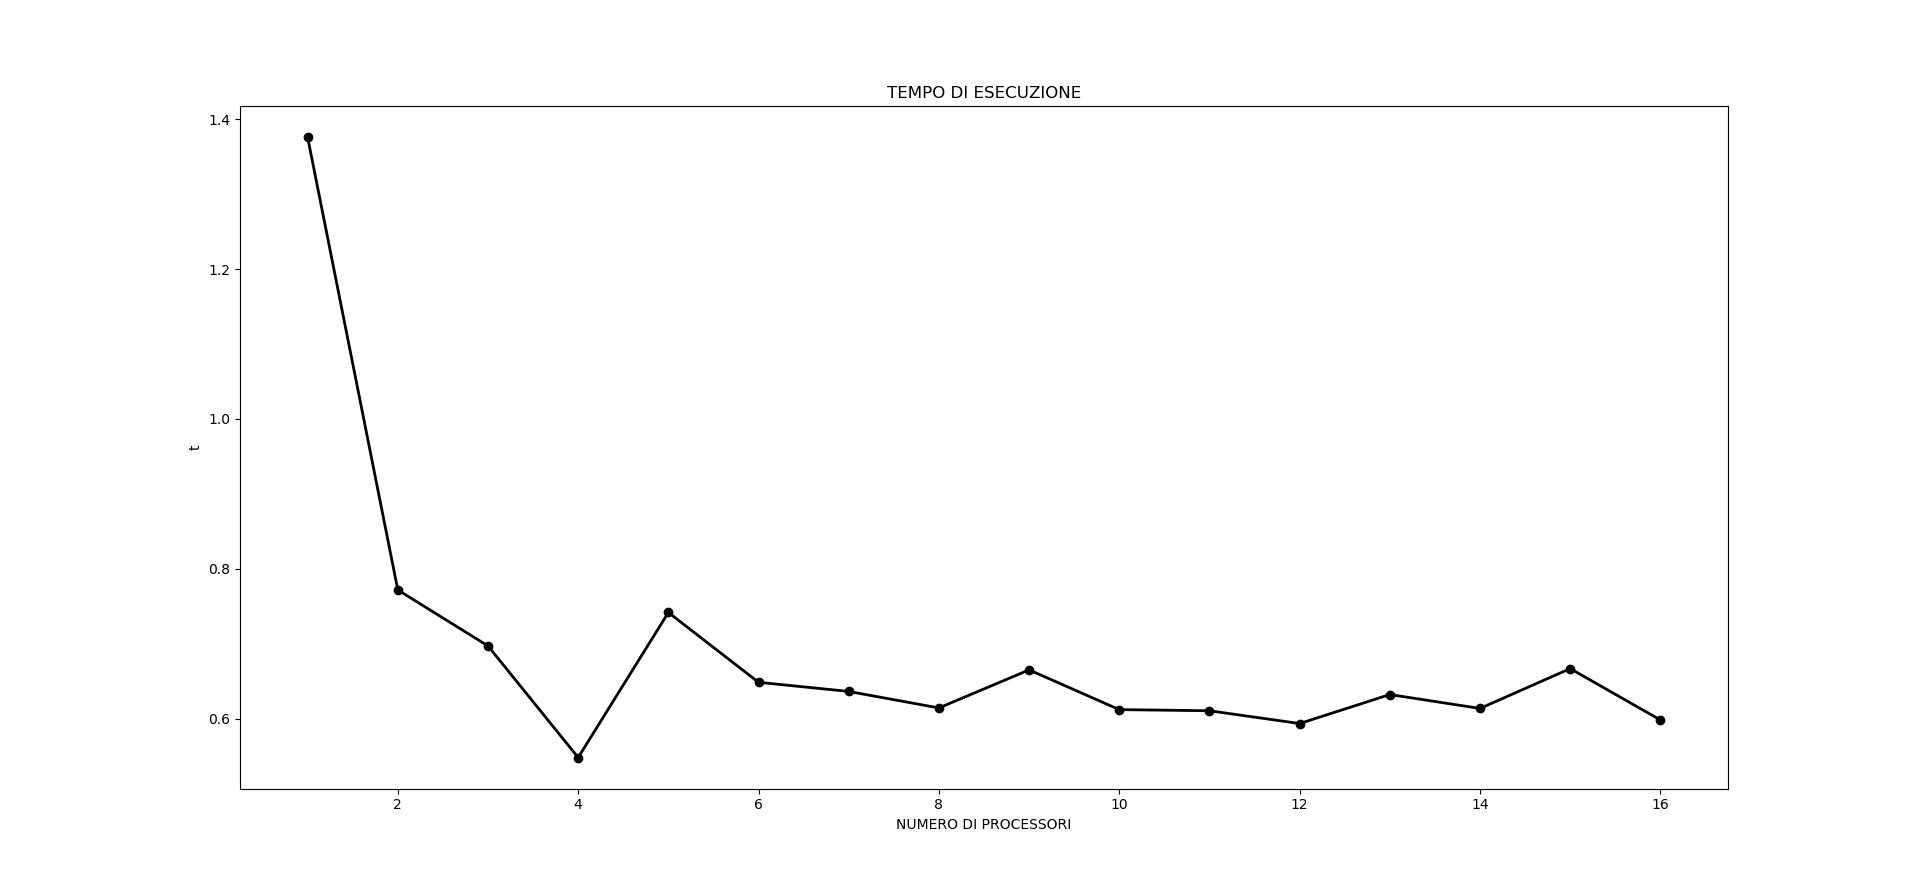
\includegraphics[width=1\linewidth]{ompt.png}
\end{figure}
Mentre l'errore  in funzione del numero di processori risulta essere identicamente uguale ad un valore dell'ordine di $10^{-3}$.
Come si può notare l'errore è indipendente dal numero di processori e lo speedup è evidente fino a 4 processori (è ciò è coerente con l'architettura usata ovvero un quad-core). Oltre tale numero si ha che il tempo di esecuzione rimane pressochè costante e si assesta sul limite teorico.
\subsection{MPI}
Lo standard MPI implementa delle librerie che permettono la comunicazione di POD (plain old data) tra più processi. I processi possono esistere nello stesso nodo o in nodi diversi e per questo motivo l'approccio si adatta anche a sistemi shared memory; la velocità di comunicazione dipende essenzialmente dalla velocità con cui possono essere trasmessi i dati. Il codice è stato pertanto eseguito sulla stessa macchina. Le strutture dati e le operazioni effettuate sono le stesse, ciò che cambia è la suddivisione del lavoro. Un processo dispone di una pozione del dominio $\Omega_s \subseteq \Omega$ e della funzione condizione iniziale. Ciò significa che ogni processo dispone di 
$$ u_0(x_i,t), x_i \in \Omega_s$$
ma non può evolvere in maniera asincrona tale soluzione perchè la derivata nei punti della frontiera $x_i \in \partial \Omega_s$ richiede la conoscenza del valore dei punti appartenenti ad un altra porzione. Ovvero 
$$u(x_i,t+1) = f(x_{i+1}, x_i, x_{i-1})$$
La condizione $x_i \in \Omega_s$ è sicuramente vera ma non necessariamente per gli altri punti. Il valore del punto sulla frontiera dovrà essere cominicato da un altro processo. Per poterlo calcolare questo processo ha però bisogno della conoscenza di un ulteriore punto del nostro dominio. Ovvero è richiesto che le porzioni del dominio debbano avere delle zone in comune, di overlap.
\newpage
\begin{figure}[H]
\centering
  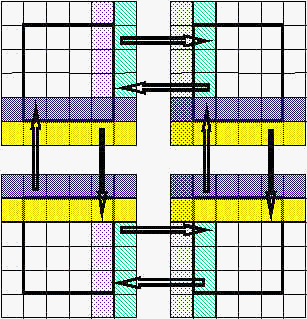
\includegraphics[width=0.5\linewidth]{ghostnodes.png}
\end{figure}
Per dieci punti e 2 processi si ha che
$$\begin{cases}
\Omega_1 = [x_0, x_1, x_2, x_3, x_4, x_5] \\
\Omega_2 = [x_4, x_5, x_6, x_7, x_0, x_1]
\end{cases}$$
Ovvero ad ogni iterazione temporale il nodo 1 deve calcolare il nuovo valore dei punti interni  $x_1, x_2, x_3, x_4$ e ricevere il valore di $x_0, x_5$ punti di frontiera (che sono infatti punti interni del dominio del nodo 2). Tale nodo dovrà anche inviare al nodo 2 il valore dei punti $x_4, x_1$.
La soluzione iniziale viene calcolata attraverso questa funzione
\begin{lstlisting}[language=C++]

\end{lstlisting}

 
\section{IL METODO DEGLI ELEMENTI FINITI}

\begin{lstlisting}[language=C++]
template <int dim>
class pdeSolver {
public:
    pdeSolver();
    void run();
private:
    void makeGrid();
    void setupSystem();
    void reinitData();
    void assembleSystem();
    int solve();
    void refineMesh(const double&, const double &,const unsigned int&, const unsigned int&);
    void executeTransferAndRefinement();
    void outputResults();
    void printRelevantInfo(const unsigned int&);
private:
    dealii::Triangulation<dim> mesh;
    dealii::DoFHandler<dim> dofHandler;
    dealii::FE_Q<dim> finiteElement;
    dealii::AffineConstraints<double> constraints;

    dealii::PETScWrappers::MPI::SparseMatrix systemMatrix;
    dealii::PETScWrappers::MPI::SparseMatrix systemRhsMatrix;
    dealii::SparsityPattern sparsityPattern;

    dealii::PETScWrappers::MPI::Vector systemRhs;
    dealii::PETScWrappers::MPI::Vector newSolution;

    dealii::Tensor<1,dim> C;
    double K{0.1};
    double time{0.0};
    double timeStep{1.0/500.0};
    unsigned int timeStepNumber{0};
    const double theta{0.50};

    unsigned int numMpiProcs;
    unsigned int thisMpiProcID;
    MPI_Comm communicator;
    dealii::IndexSet numOwnedDofs;
};
\end{lstlisting}




\end{document}
